\documentclass[a4paper,10pt,openright,oneside,notitlepage]{report}

\usepackage[utf8]{inputenc}
\usepackage[ngerman]{babel}
\usepackage{hyperref}
\usepackage[toc,acronym]{glossaries}
\usepackage[square, numbers]{natbib}
\usepackage{graphicx}
\usepackage{float}

\title{Anforderungsanalyse der Bachelorarbeit}
\author{Daniel Pollack}
\date{}

\newcommand{\ProgrammName}{ProgrammnamePlatzhalter}

\pdfinfo{
  /Title    (\title)
  /Author   (\author)
  /Creator  (\author)
  /Producer (\author)
  /Subject  (Anforderungsanalyse)
  /Keywords (Anforderungsanalyse, Arduino, C#, C sharp, Gtk, Bachelorarbeit)
}

\makeglossary


\begin{document}
\maketitle
\tableofcontents

\chapter{Einleitung}
\section{Anlass}
Die Idee zu diesem Bachelorthema ist aus dem Arbeitsalltag am Max-Plack Institut
für Biogeochemie in Jena entstanden. Durch Gespräche mit Kollegen und beim
\gls{Brainstorming} mit meinem Vorgesetzten bin ich zu dem Entschluss gekommen, 
dass das angestrebte Thema eine sinnvolle Ergänzung im Arbeitsalltag und eine
Verbesserung der Arbeitsabläufe, sowohl im Institut als auch anders wo
darstellt.

\section{Zweck}
Zweck dieser Arbeit soll es sein, eine Software zu entwickeln die den Aufbau und
die Wartung von Versuchsaufbauten beschleunigt und vor allem vereinfacht. Bei meiner Recherche stellte sich heraus, dass manche der am Institut
verwendeten Systeme lediglich von einer geringen Anzahl Personen konfiguriert und gewartet werden können. Dieser Zustand ist keineswegs optimal und kann, z.B. durch das Fernbleiben eben dieser Personen, den betrieblichen Ablauf erheblich stören.
\section{Ziele}
Diese Arbeit hat zum Ziel eine Softwarelösung zu entwickeln und umzusetzen, die 
es einem elektrotechnisch geschulten und in dem Umgang mit Computern geübten 
Nutzer erlaubt einen elektronischen Schaltkreis zu überwachen, zu messen und zu 
steuern. Dem Nutzer soll eine Möglichkeit geboten werden, mittels eines eingängigen Interfaces, Messungen an elektrotechnischen Schaltungen vor zu nehmen. Darüber hinaus soll die Erstellung von Schaltvorgängen in einer elektrotechnischen Schaltung ermöglicht werden.
\section{Referenzen}
Bei Recherchen verfestigte sich mein Eindruck, dass eine solche Software durch aus das Potential besitzt, Wissenschaftlern und \gls{Maker}[n] das Leben und ihre Arbeit zu vereinfachen. So ist das Interesse an erschwinglicher Hardware und handlicher 
Software zum Prototyping und dem Aufbau von Versuchen besonders durch das 
Aufkommen des Arduinos gewachsen. D.~K.~Fisher und P.~J.~Gould~\cite{ModernInstrumentation} beschrieben in ihrem Paper einen 
Versuchsaufbau mit Hilfe eines Arduino-Nachbaus zur Ermittlung von 
Feuchtigkeitswerten in und um Pflanzen herum. Ihr Aufbau und vorallem die 
Software verfolgen ein ähnliches Prinzip wie das von mir angestrebte. Der 
Arduino dient ihnen als Datenerfassungsergrät und übermittelt alle Daten ohne 
weitere Verarbeitung direkt an entweder ein Speichermedium oder an einen 
Server. In diesem und einigen anderen Papers geht es häufig auch um eine finanzielle Sicht auf Experimente und die damit verbundene Durchführbarkeit. So beschreibt \citet{joshua_m._pearce_open-source_2014} in Kapitel 4 seines Buches, wie er eine Feuchtigkeitskammer für seine Forschungsarbeit anschaffen wollte. Er beschreibt, dass die kommerziell verfügbaren Produkte außerhalb des gegebenen Finanzrahmens waren und man somit auf eine \acrshort{DYI}-Lösung zurückgreifen musste. kern dieser Lösung war, aufgrund seines Preises und der beständigen Unterstützung durch Software-Bibliotheken Dritter, der Arduino.

Der Aspekt einer Datenerfassung und Auswertung hat bereits Andere veranlasst 
eine entsprechende Lösung inklusive Software zu erstellen. Einer der jüngeren Ansätze stammt 
aus der Universität Basel~\cite{Instrumentino} und umfasst eine Software 
(Instrumentino) mit deren Hilfe extra angefertigte Arduino-Sketche (Controlino) 
und eine problembezogen konfigurierte Oberfläche zum Einsatz kommen. 
Nach eindringlicher Analyse der Software und einem Versuch eine eigene 
Testkonfiguration mit der Software und unter Zuhilfenahme des Entwicklers zu erstellen, bin 
ich zu dem Schluss gekommen, dass diese Software nicht als ausgereift angesehen 
werden kann und nur unter Einsatz kundiger Personen, bezüglich der grundlegenden Einrichtung einzelner Versuchsaufbauten, zum Einsatz gelangen kann. Der Entwickler weißt in einer 
\href{https://github.com/yoelk/Instrumentino/blob/master/documents/Instrumentino\%20presentation.pptx}{Präsentation} auch darauf hin, dass der Konfigurationsprozess einen "`Administrator/Entwickler"' benötigt und es nicht vorgesehen ist diesen Schritt einem Endnutzer zu überlassen. 
Ein ausgereiftes Konzept, wenn auch etwas älter stammt von \citet{dedrick_inexpensive_2000} und beschreibt einen Datenlogger auf Mikrocontrollerbasis mit einer entsprechenden Software zum Auslesen der gesammelten Daten. Auch hier wurde Wert auf den finanziellen Rahmen, sowie die Weiterverarbeitung und Langzeiterfassung von Daten gelegt. Allerdings liegt der Fokus mehr auf einer Anwendung in abgelegenen Regionen und der damit verbundenen anschließenden Auswertung der Daten. Folglich wurde bewusst auf eine Echtzeitüberwachung verzichtet.
\chapter{System}
\section{Übersicht}
%Beschreibung Programm
Das System besteht aus zwei Teilen. Der eine Teil besteht aus einer Desktop Computer Anwendung und der zweite Teil  aus einem Arduino-Sketch.
Beide Teile erfahren in den folgenden Abschnitten eine genauere Beschreibung. Vorweg soll lediglich der generelle Aufbau des Systems umrissen werden.

Die Desktop Computer Anwendung soll dem Nutzer eine Oberfläche bieten, mit der er ohne Programmierkenntnisse einen Messungs- und Steuerungsaufbau für den Arduino erstellen und verwalten kann. Die Oberfläche soll bei einer erfolgreichen Erstellung und Ausführung in Echtzeit die Daten visualisieren und gleichzeitig in eine, vom Nutzer vor Beginn der Messung konfigurierte, \acrshort{CSV}-Datei speichern.

Der Arduino-Sketch wird eine Logik bekommen, mit der es möglich sein wird seine Ein- und Ausgänge während der Laufzeit anusprechen. Diese Vorgehensweise ermöglicht es, abgesehen von etwaigen Software-Updates, dass Neueinrichtung und das Aufspielen eines Arduino-Sketches einmalig notwendig sein wird. Anschliessend kann der mit dem Sketch gebrannte Arduino in allen kommenden Versuchsaufbauten verwendet werden, ohne des eine neue Software installiert werden muss. Dis kommt weniger geschulten Nutzern entgegen und erspart ihnen eine Auseinandersetzung mit der Arduino \acrshort{IDE}.

%ToDo Bild

\section{Funktionalitäten}
Folgende Funktionalitäten sollen in dieser Arbeit umgesetzt werden:
\begin{itemize}
 \item Umsetzung eines Nutzerfreundlichen Interfaces
 \item vereinfachtes Aufsetzen des Systems
 \subitem Dies bezieht sich vor allem auf die Einrichtung des Arduinos
 \item Echtzeitloggen beliebiger Messwerte in beliebigen Frequenzen
 \item Echtzeitvisualisierung der Messergebnisse
 \item Angabe von \gls{Uebertragungsfunktion} für einzelne Signale + Visualisierung
 \item Konfigurierbarkeit der Visualisierung
 \item Erarbeitung eines Protokolls für die Mikrocontroller - PC Kommunikation
 \item Datenlogger mit angemessen hohem Grad an Konfigurationsmöglichkeiten
\end{itemize}

\section{Optionale Funktionalitäten}
\begin{itemize}
 \item Das Interface bietet die Möglichkeit zum Aufspielen des Arduino-Sketches (z.B. ein ``Uploadbutton'')
 \item Unterstützung mehrerer Arduino-Produkte und Chipsätze
 \item Unterstützung von Protokollen wie etwa I2C
 \item Visualisierungen können abgekoppelt vom Hauptfenster auf dem Desktop angeordnet werden
 \item Eventlogging \gls{Eventlogging} soll ermöglicht werden.
 \item Update-Benachrichtigung
\end{itemize}

\section{Nutzer}
Die angestrebte Zielgruppe dieses Systems kennt sich mit Elektrotechnik aus und ist vertraut mit der Bedienung von Computern und darauf installierten Anwendungen. Ein wissenschaftlicher Hintergrund ist von Vorteil, aber nicht notwendig. Das System soll sich sowohl an Forscher, als auch \gls{Maker} richten.
Eine Alterseinstufung ist nicht notwendig. Die persönliche Befähigung ist ausschlaggebend für eine erfolgreiche Nutzung.

\section{Interface / Usability}
Um eine gute Usability für den Nutzer zu gewährleisten, werden weitestgehend Interface Elemente verwendet die der Nutzer bereits aus anderen Anwendungen und Systeme her kennt.
Dies bezieht sich besonders auf grafische Schemata der Betriebssystemeigenen Elemente. %Dieses Schema soll nach Möglichkeit übernommen werden.

Der Ablauf und der Aufbau des Interfaces soll eine Pipeline-Struktur ergeben, um dem Nutzer eine geführte Konfiguration eines Versuchsaufbaus zu ermöglichen. Sollte der Nutzer bereits mit der Bedienung anderer Anwendungen und Systeme vertraut sein, hat er allerdings auch die Möglichkeit aus dieser Pipeline auszubrechen und sich eine eigene Schrittfolge anzueignen. Vergleichen kann man dieses Pipeline-Design mit einem Installationsassistent, der dem Nutzer Schritt für Schritt einzelne Aspekte der Konfiguration zeigt, ohne den Nutzer mit momentan nicht relevanten Informationen zu überfordern.

Für die Erarbeitung wird ein High-fidelity Prototyping mittels eines interaktiven Computer-Prototyps angestrebt. Die Entscheidung für diese Vorgehensweise lässt sich mit dem hohen Maß an Interaktivität für den Nutzer beschreiben. Bedenken bezüglich eines höheren Aufwandes sind gerechtfertigt, jedoch überwiegen die Vorteile. Der Nutzer kann in einer ihm vertrauten, und vor allem der angestrebten, Umgebung den Prototypen verwenden. Die im Interface verwendeten Elemente sehen dabei bereits so aus wie im Endprodukt.Somit können Abstraktionsunterschiede und eine Eingewöhnungszeit minimiert werden. Im Vergleich zu einem Papermockup oder einer Evaluation mittels Szenario kann mit der angestrebten Methode gezielter auf die geplanten Funktionalitäten getestet werden. Abgesehen davon gibt es allerdings keine größeren Unterschiede zwischen den verfügbaren Methodiken~\cite{johansson_case_2007}. Berücksichtigt man allerdings die Zielgruppe dieser Arbeit, liegt eine weniger abstrakte und daher interaktiver Prototyping-Methode nahe. 

Zusätzlich lässt sich mit dieser Art von Prototyp eine detailliertere Evaluation vornehmen, durch z.B. genauere Zeitmessung für die Erfüllung einzelner Teilaufgaben. Beispielsweise kann genauer gemessen werden wie lange ein Nutzer braucht um eine Option zu aktivieren. Die Erkenntnisse der Evaluation können, so fern nicht schwerwiegend, direkt in der Oberfläche integriert werden.
\section{Verlässlichkeit / Wartung}
Im Vordergrund dieser Arbeit steht die erfolgreiche Umsetzung der Idee in Form einer Implementation. Eine längerfristige Wartung und Weiterentwicklung des Systems ist daher momentan nicht von vorrangigem Interesse. Es sei jedoch auf die Lizenzierung zu verweisen, in der eine Open-Source Lizenz angestrebt wird. Zu dem sollen alle relevanten Dokumente einschließlich des Quellcode auf einer frei zugänglichen Plattform veröffentlicht werden.
Denkbar ist in diesem Falle die Seite \href{https://github.com/}{GitHub}, welche sich durch eine große Community auszeichnet und die Kontrolle und Verwaltung eines Projekte ermöglicht. Auch ein Feedback-Kanal und eine transparente Entwicklung werden ermöglicht. So können Nutzer direkt mit dem Entwickler in Verbindung treten und gefundenen Fehler ("`Bugs"'), sowie Feature-Vorschläge direkt unterbreiten und miteinander Diskutieren.

Für Fragen der Nutzer, besonders bei Problemen, kann ein \acrshort{FAQ} eingerichtet werden. Für speziellere Problem steht dem Nutzer auch der direkte Kontakt zur Verfügung.
%\section{Leistung}
\section{Implementation / Umsetzung}
Die Umsetzung der Desktop Computer Anwendung wird in der Sprache \href{http://www.mono-project.com/}{Mono} geschehen. Für die Grafische Benutzeroberfläche wird die Bibliothek \href{http://www.gtk.org/}{GTK-sharp} in der Version 2.12 verwendet. Der Arduino-Sketch wird in C++ implementiert.

Um eine problemarme Umsetzung zu gewährleisten ist es von äußerster Wichtigkeit, die zugrunde liegenden Softwarekomponenten im Vorfeld ausreichend zu testen und sich mit ihnen vertraut zu machen. 
%ToDo 
\section{Packaging}
Ein Packaging gestaltet sich als etwas anspruchsvoller, da mehrere Betriebssystem berücksichtigt werden müssen. Für den Vertrieb auf Unix/Linux System ist es gängige Praxis die Software in einem entsprechenden Containerformat in einem der Repositories zu hinterlegen. Diese Methode hat den Vorteil eines dem Nutzer vertrauten Installationsprozesses und sichert weiterhin, sofern regelmäßig vom System oder Nutzer initialisiert, die Aktualität der Software. 
Für Windows existiert so eine Repository-Lösung, nativ, bisher nicht. Es werden daher Architektur spezifische Binärdateien erstellt und auf der gewählten Internetpräsenz zum Download angeboten. 
Es wird für jedes gängige System ein Handbuch erstellt, um einen geführten Installationsprozess zu gewährleisten.
Die Installation von Dritt-Software wird nicht übernommen. 

Jedoch ein Hinweis im Handbuch und bei dem Installationsprozess auf fehlende Komponenten wird erfolgen.

Alternativ kann die Software auch direkt von ihrer Internetseite bezogen werden und vom Nutzer selbstständig installiert werden.
\section{Lizenz}
Eine Auswahl für eine endgültige Lizenz muss noch getroffen werden. Unter Berücksichtigung der beteiligten Partei muss eine Lösung gefunden werden. Persönlich strebe ich eine Open-Source Lösung an.
Bei der Wahl der Lizenz muss die verwendete Software Dritter berücksichtigt werden. Manche Lizenzen, wie zum Beispiel die \href{https://www.gnu.org/licenses/licenses.html#GPL}{GNU-Lizenz}, vererben sich und lassen somit nur wenige Optionen offen: 1. Verwendung der Dritt-Software, 2. Implementierung einer eigenen Lösung oder 3. Verwendung einer anders lizenzierten Alternative.
\section{Zu klärende Fragen}
\begin{itemize}
 \item Interface
  \subitem Sichtung von Plotbiblotheken
  \subitem Nutzerbefragung zu Mockups
 \item Kommunikation
  \subitem Sichtung von Arduino-PC Bibliothek  
\end{itemize}



\chapter{Modelle}
\section{Szenarios}
\subsection{Überwachung und Messung an einem Versuchsaufbau}
\subsection{Steuerung und Messung an einem Versuchsaufbau}
\section{Use case model}
Dieses Use case Diagramm zeigt die dem Nutzer zu Verfügung stehen Optionen.
\begin{figure}[H]
 \centering
 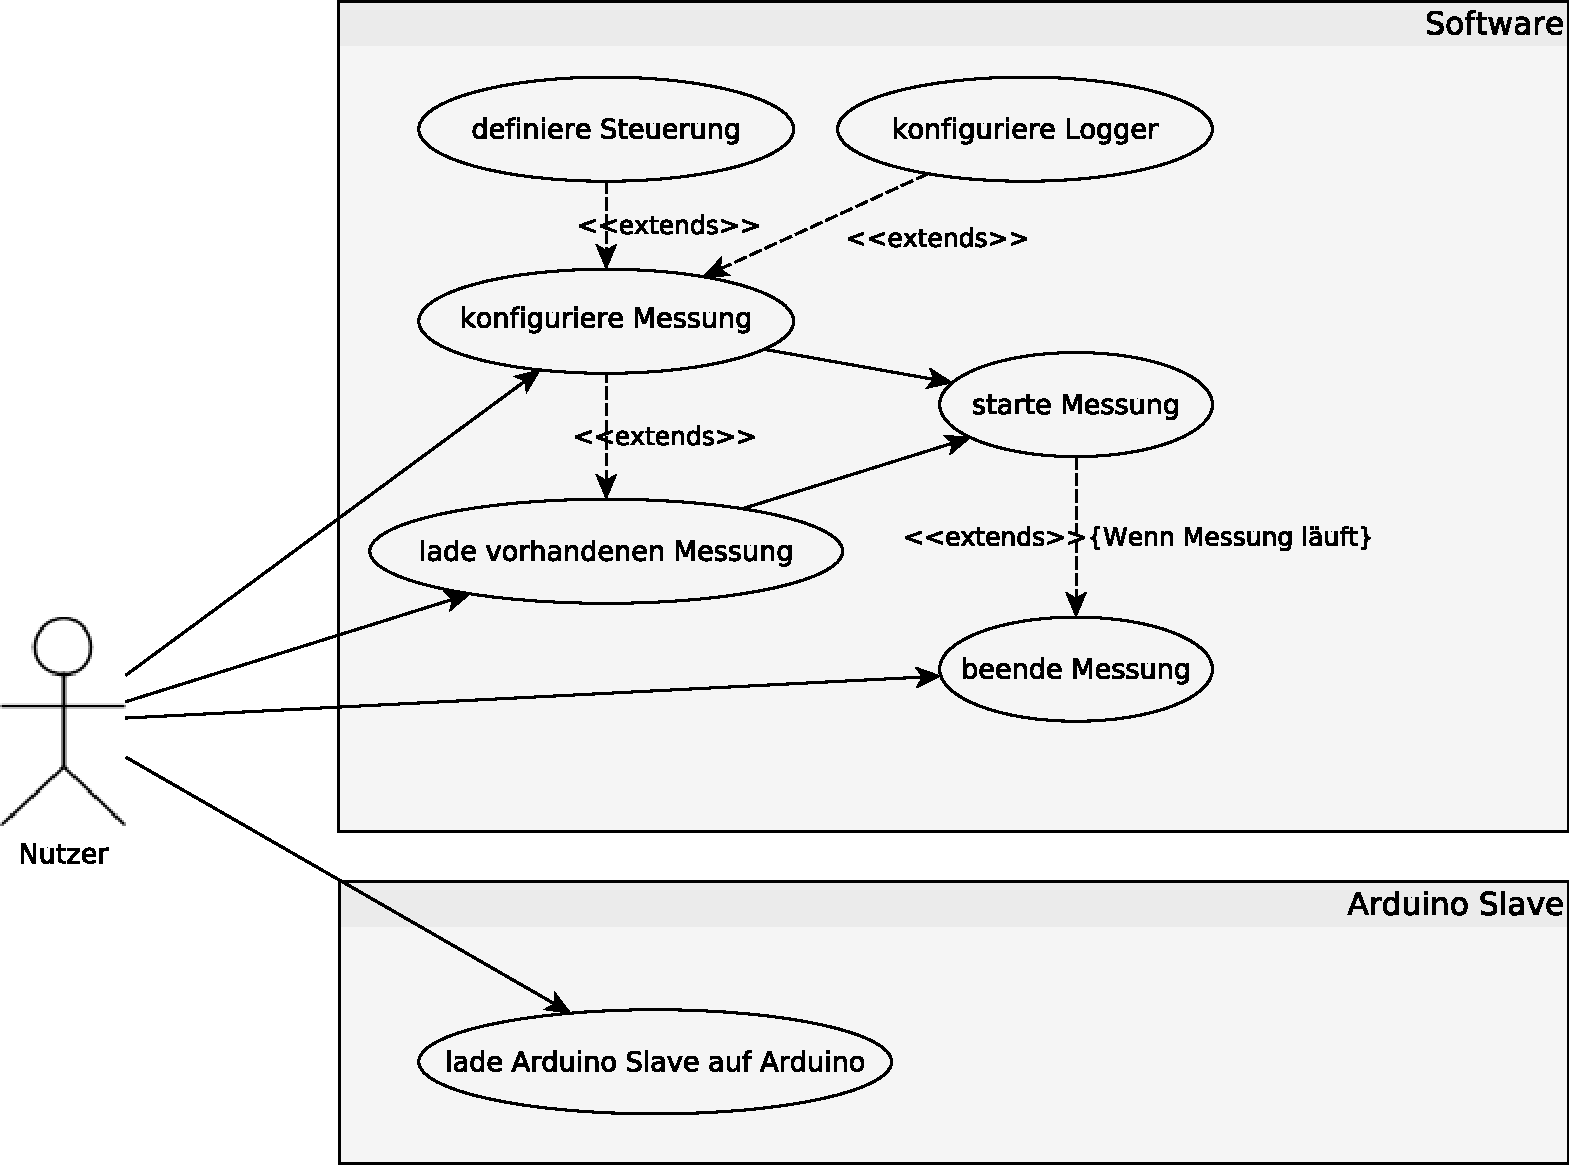
\includegraphics[width=\textwidth, keepaspectratio=true]{../Diagramme/BachelorUseCase1.pdf}
\end{figure}

%\section{Analysis object model}
%\section{Dynamic model}
\section{Flowchart}
Dieses Flowchart zeigt die notwendigsten Schritte, die von der Software und dem Nutzer unternommen werden müssen um eine erfolgreiche Messung durch führen zu können. 
\begin{figure}[H]
 \centering
 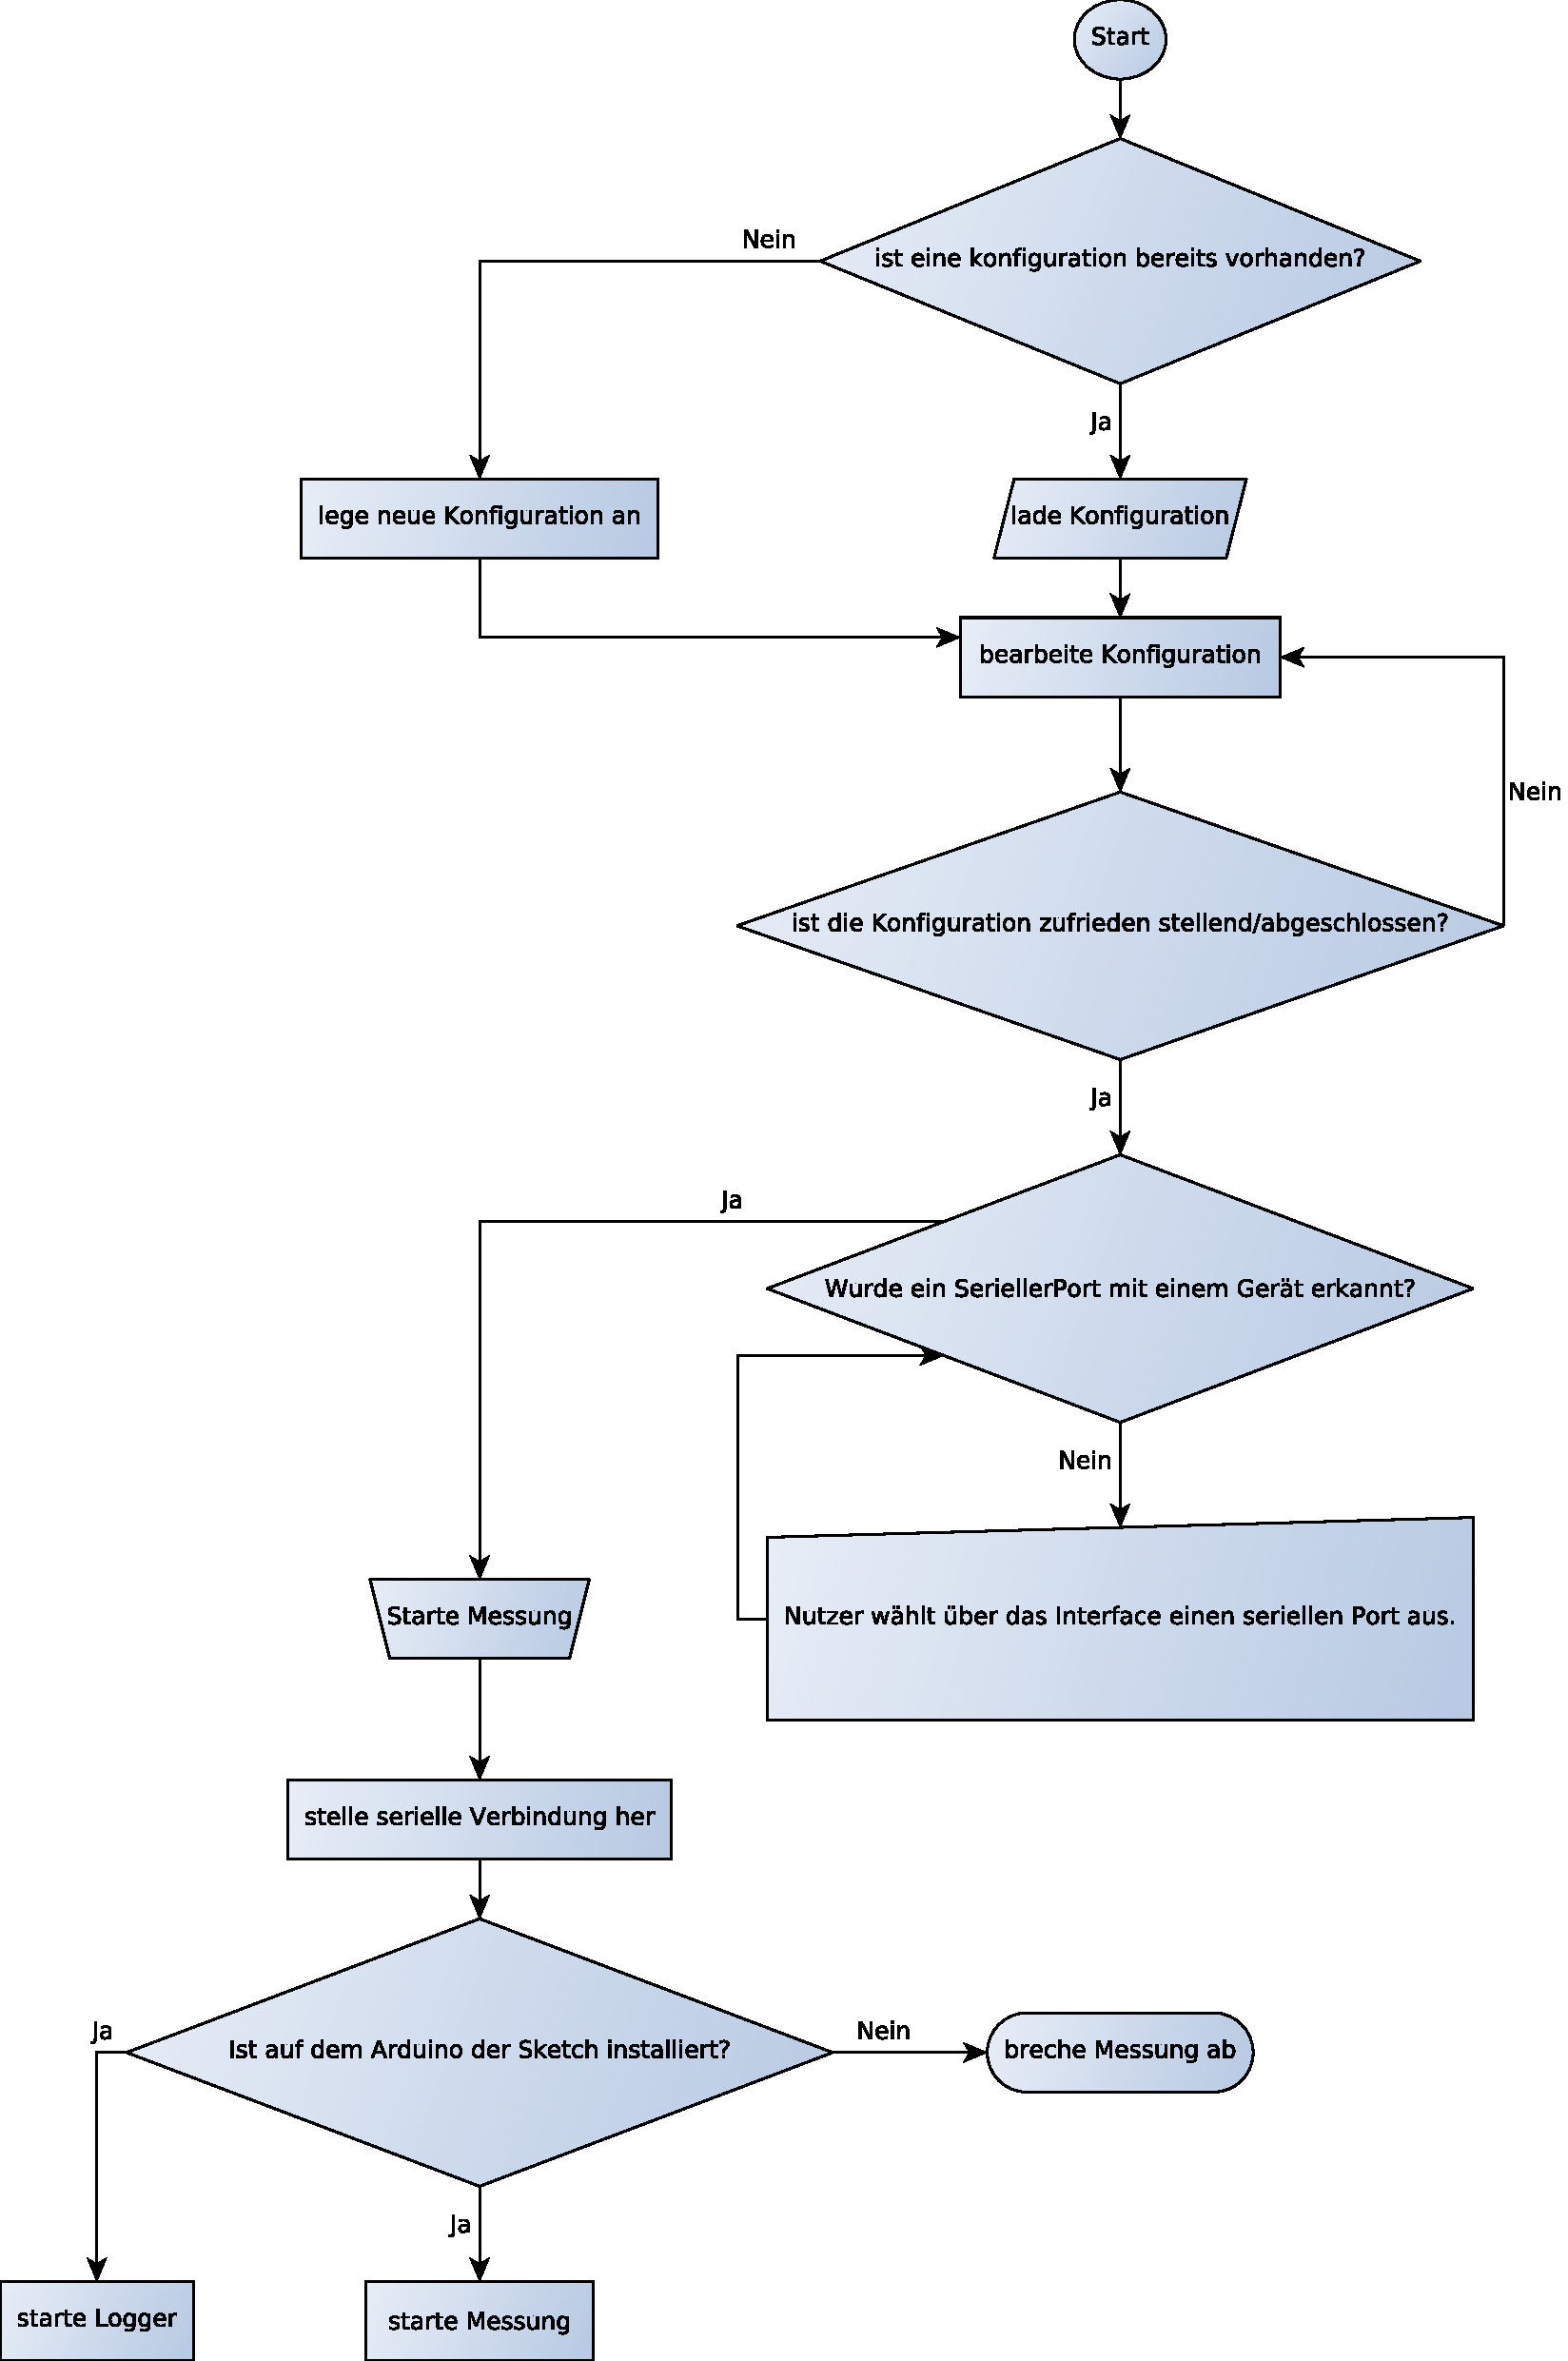
\includegraphics[width=\textwidth, keepaspectratio=true]{../Diagramme/SoftwareFlowChart.pdf}
\end{figure}
\section{Aufbau}
%grobes UML
\section{User Interface - Navigation und Mockups}
%\addcontentsline{toc}{chapter}{Glossar}
\newglossaryentry{Brainstorming}{
name=Brainstorming,
description={Eine Methode zur Findung von neunen, ungewöhnlichen Ideen}
}
\newglossaryentry{Maker}{
name=Maker,
description={Eine Person die zu der 'Do-It-Yourselfe' Subkultur zählt und Geräte/Maschienen unter Einsatz moderner Technik herstellt}
}
\newglossaryentry{Eventlogging}{
name=Eventlogging,
description={Ermöglicht die Protokollierung von (vordefinierten) systembezogenen Event. Dies ist dienlich für die Analyse eines System}
}
\newglossaryentry{Uebertragungsfunktion}{
name=Übertragungsfunktion,
description={Eine Übertragungsfunktion beschreibt im naturwissenschftlichen Rahmen eine Funktionen die den Zusammenhang zwischen Eingangs und Ausgangssignal beschreibt}
}
\newacronym{FAQ}{FAQ}{Frequently Asked Questions}

\newglossaryentry{CSV-detail}{
name={Comma-separated values},
description={Ein plain-text Format, in dem Werte durch Kommata getrennt gespeichert werden}
}
\newacronym[see={[Glossary:]{CSV-detail}}]{CSV}{CSV}{Comma-separated values\glsadd{CSV-detail}}
\printglossaries

\addcontentsline{toc}{chapter}{Bibliography}
\bibliographystyle{plainnat}
\bibliography{Bibliography}


\end{document}
